\subsection{Conditioning: Robustness Through Template Dropout}
\label{sec:recipe-conditioning}

\textbf{Explored designs.}
Because available conditioning information varies across targets, a single model should handle different subsets of optional inputs. We vary
the template-coordinate dropout probability
$p_{\mathrm{tpl}}\in\{0,0.5,1\}$ and evaluate each model under five
inference-time conditioning settings: none, stereochemistry only, template only,
stereochemistry plus template, and all three conditions including space group.

\textbf{Results and selection.}
Moderate template dropout ($p_{\mathrm{tpl}}=0.5$) is the most robust across
conditioning settings, achieving the highest mean $\mathrm{Sol}_C$ over the five
settings ($0.487$, compared with $0.483$ and $0.264$ for
$p_{\mathrm{tpl}}=0$ and $1$, respectively). Notably, exposure to templates
during training also improves performance when no optional conditioning is
provided: $p_{\mathrm{tpl}}=0.5$ reaches $0.459$, compared with $0.442$ for a
model that never observes templates. We therefore select
$p_{\mathrm{tpl}}=0.5$ (\Cref{fig:conditioning-sweep}).

\begin{figure}[!t]
  \centering
  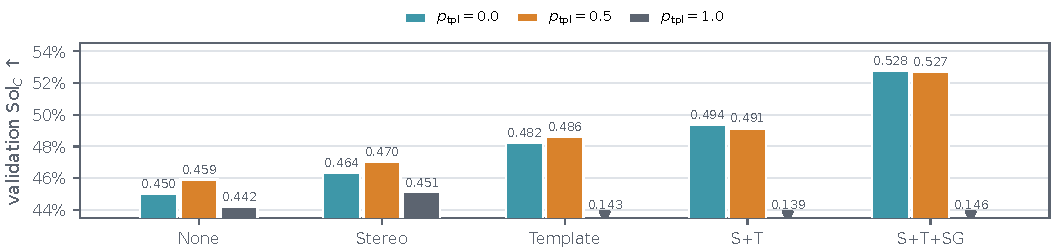
\includegraphics[width=\textwidth]{figures/generated/fig_conditioning_sweep.pdf}
  \caption{\textbf{Moderate template dropout is most robust across conditioning
    settings.} Validation $\mathrm{Sol}_C$ at epoch 300 using EDM--Heun with
    200 steps and 30 candidates per target. S, T, and SG denote stereochemistry,
    template coordinates, and space-group conditioning, respectively. Among
    models trained with $p_{\mathrm{tpl}}\in\{0,0.5,1\}$,
    $p_{\mathrm{tpl}}{=}0.5$ achieves the highest average performance across the
    five inference-time conditioning settings and is therefore selected.
    Template-conditioned results for $p_{\mathrm{tpl}}{=}1$ fall below the
    plotted range and are shown as downward triangles.}
  \label{fig:conditioning-sweep}
\end{figure}